%% LyX 2.1.4 created this file.  For more info, see http://www.lyx.org/.
%% Do not edit unless you really know what you are doing.
\documentclass[british]{beamer}
\usepackage{ccfonts}
\renewcommand{\familydefault}{\rmdefault}
\usepackage[T1]{fontenc}
\usepackage[latin9]{inputenc}
\setcounter{secnumdepth}{3}
\setcounter{tocdepth}{3}
\usepackage{url}
\usepackage{amsmath}
\usepackage{amssymb}
\usepackage{graphicx}

\makeatletter
%%%%%%%%%%%%%%%%%%%%%%%%%%%%%% Textclass specific LaTeX commands.
 % this default might be overridden by plain title style
 \newcommand\makebeamertitle{\frame{\maketitle}}%
 % (ERT) argument for the TOC
 \AtBeginDocument{%
   \let\origtableofcontents=\tableofcontents
   \def\tableofcontents{\@ifnextchar[{\origtableofcontents}{\gobbletableofcontents}}
   \def\gobbletableofcontents#1{\origtableofcontents}
 }

%%%%%%%%%%%%%%%%%%%%%%%%%%%%%% User specified LaTeX commands.
\bibliographystyle{apsrev4-1}

\makeatother

\usepackage{babel}
\begin{document}

\title{Contextuality in a Deterministic Theory}


\date{January 15, 2016}
\makebeamertitle
\begin{frame}{Thesis Problem}

\begin{itemize}
\item Two theories: Quantum Mechanics (QM) \& Bohmian Mechanics (BM)
\end{itemize}

\pause{}
\begin{itemize}
\item Fundamental difference: BM is deterministic, viz. positions ($q$)
and momenta ($p$) are well defined
\end{itemize}

\pause{}
\begin{itemize}
\item Aim: Construct a theoretical situation that defies determinism using
QM and analyze using BM
\end{itemize}
\end{frame}

\begin{frame}{Overview of the talk}

\begin{itemize}
\item Bohmian Mechanics (BM)
\end{itemize}

\pause{}
\begin{itemize}
\item Determinism: The GHZ test \& Contextuality
\end{itemize}

\pause{}
\begin{itemize}
\item Its analysis using BM
\end{itemize}

\pause{}
\begin{itemize}
\item {[}recent{]} Determinism in phase space ($q$,$p$)
\end{itemize}

\pause{}
\begin{itemize}
\item {[}in progress{]} Its analysis using BM
\end{itemize}
\end{frame}

\begin{frame}{}


{\Huge{Bohmian Mechanics (BM)}} \\
Determinism \& Contextuality \\
Its analysis using BM \\
(recent) Determinism in phase space $(q,p)$ \\
(in progress) Its analysis using BM

\end{frame}

\begin{frame}{Bohmian Mechanics (BM)}

\begin{itemize}
\item QM: `Copenhagen interpretation'; how to verify?
\end{itemize}

\pause{}
\begin{itemize}
\item D. Bohm: `hidden variable' theory

\begin{itemize}
\item in principle known, in practice averaged
\end{itemize}

\pause{}

\item Lessons:

\begin{itemize}
\item Clarity: (a) description (b) deriving classical mechanics
\end{itemize}

\pause{}
\begin{itemize}
\item Accuracy of deductions: (a) Bell test (b) GHZ/Determinism test
\end{itemize}

\pause{}

\item Immediate questions: (a) Uncertainty principle (b) Double slit, which
is chosen? (c) Trajectories; observable? (d) Identical particles
\end{itemize}
\end{frame}

\begin{frame}{BM | Formalism}


A particle is associated with (1) $(q,p)$, which are precisely and
continuously defined \& (2) a wave $(\psi)$. If the following are
assumed, all results of QM are reproduced:


\pause{}
\begin{itemize}
\item $\psi$ satisfies the Schr\"odinger equation
\end{itemize}

\pause{}
\begin{itemize}
\item $mv=p=\nabla S=\hbar\text{Im}(\nabla\psi/\psi)$, where $\psi=Re^{iS/\hbar}$
\end{itemize}

\pause{}
\begin{itemize}
\item in practice, we have a statistical ensemble with probability densities
$\rho(q)=\left|\psi(q)\right|^{2}$
\end{itemize}
\end{frame}

\begin{frame}{BM | Formalism}


Comments:
\begin{itemize}
\item Observers not fundamental; $\hbar=0$
\end{itemize}

\pause{}
\begin{itemize}
\item Ready generalization to $N$ particles. Non-locality becomes explicit;
$p_{i}=\nabla_{i}S(q_{1},q_{2},\dots,q_{N})$
\end{itemize}

\pause{}
\begin{itemize}
\item Extension to spins: Particle has $(q,p)$. The wavefunction has the
spinor, say $\Psi\equiv(\psi_{+},\psi_{-})^{T}$; the generalization
is 
\[
p=mv=\hbar\text{Im}\frac{(\Psi,\nabla\Psi)}{(\Psi,\Psi)}
\]
where $(.,.)$ is the inner product in the spin space $\mathbb{C}^{2}$.
\end{itemize}
\end{frame}

\begin{frame}{BM | Pictures}


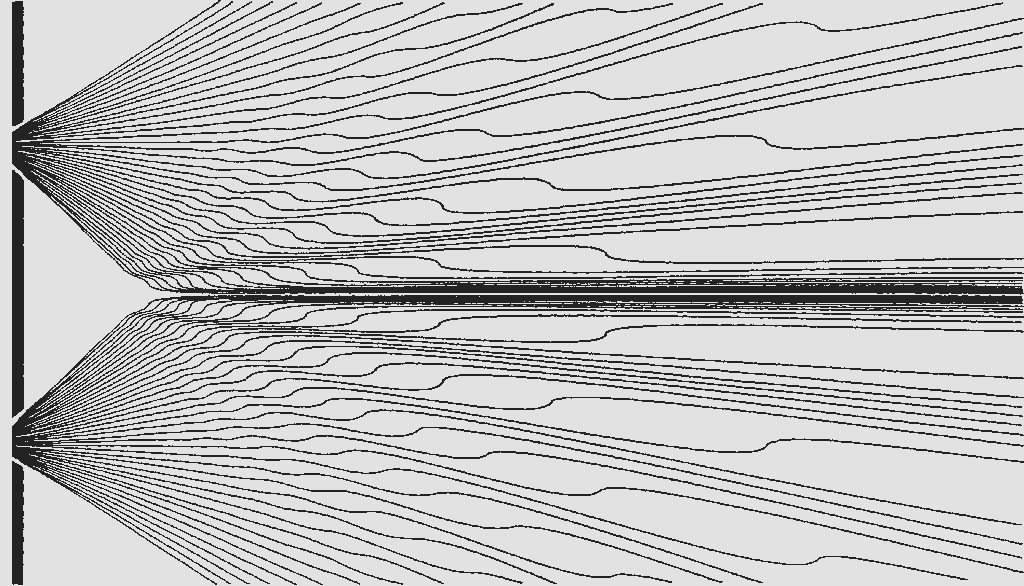
\includegraphics[width=10cm]{images/doubleSlit}


\end{frame}

\begin{frame}{BM | Pictures}


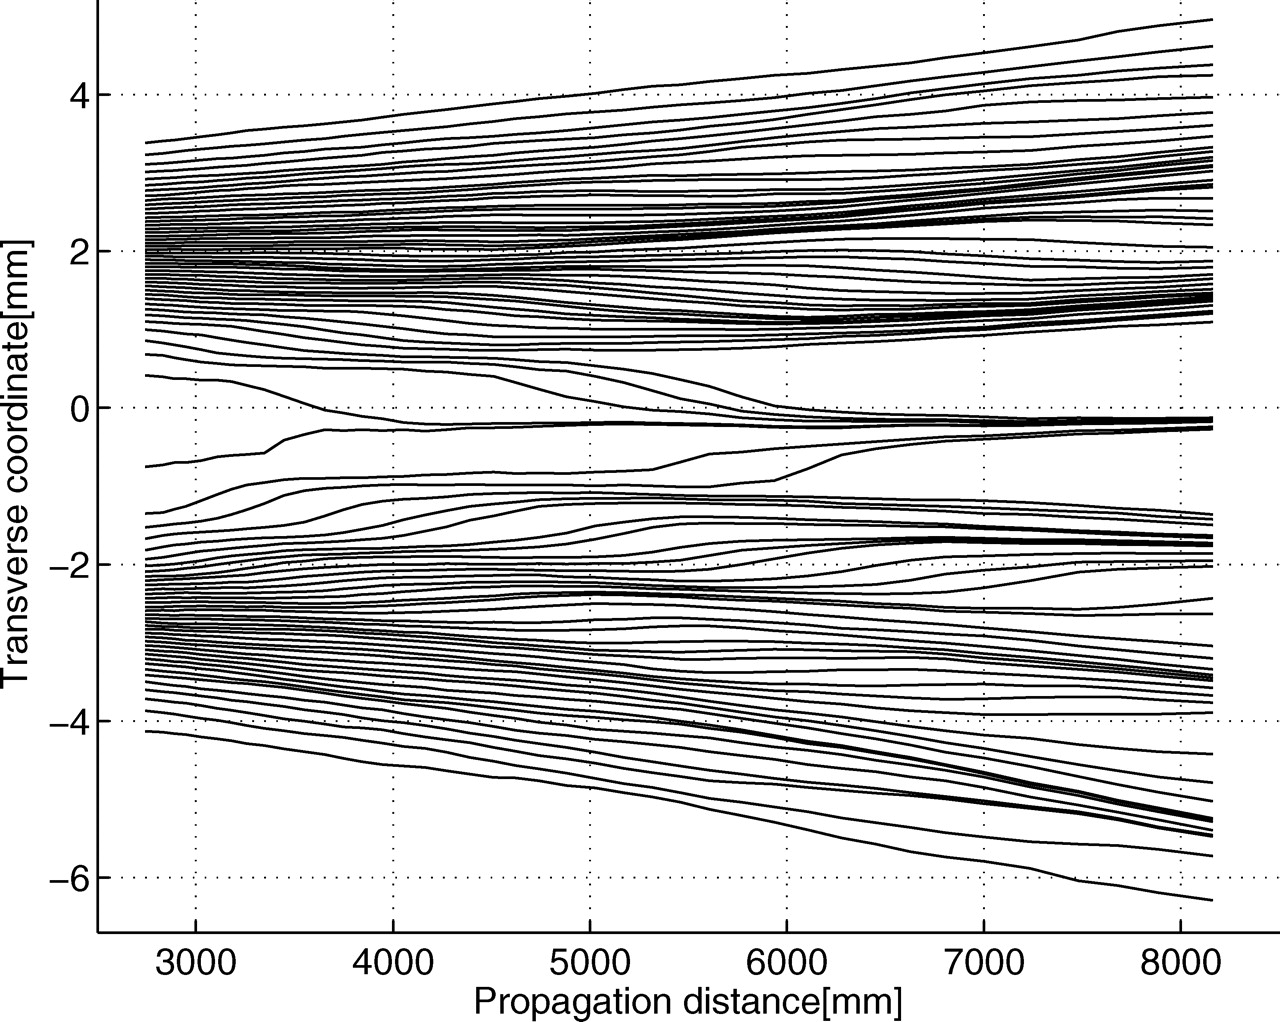
\includegraphics[width=6cm]{images/expDoubleSlit}

``Observing the Average Trajectories of Single Photons in a Two-Slit
Interferometer''
\end{frame}

\begin{frame}



Bohmian Mechanics (BM) \\
{\Huge {Determinism \& Contextuality}} \\
Analysis using BM \\
(recent) Determinism in phase space $(q,p)$ \\
(in progress) Its analysis using BM


\end{frame}

\begin{frame}{Determinism}


Defn: Determinism: Observables have values regardless of whether they
are measured, viz. values are predefined.

\end{frame}

\begin{frame}{Determinism: The GHZ Test (1/2)}

\begin{itemize}
\item Objective: To show that the notion of determinism is incompatible
with QM.
\end{itemize}

\pause{}
\begin{itemize}
\item Assume: 


\pause{}
\begin{itemize}
\item Three particles; interact initially; given to three observers (one
each)
\end{itemize}

\pause{}
\begin{itemize}
\item Two properties, $\hat{X}$ \& $\hat{Y}$, outcome is $\pm1$
\end{itemize}

\pause{}

\item General Construction: $\hat{A}\equiv\hat{X}\otimes\hat{Y}\otimes\hat{Y}$,
$\hat{B}\equiv\hat{Y}\otimes\hat{X}\otimes\hat{Y}$ and $\hat{C}\equiv\hat{Y}\otimes\hat{Y}\otimes\hat{X}$;
outcome is $+1$ for each. $\hat{D}\equiv\hat{X}\otimes\hat{X}\otimes\hat{X}$
yields $-1$. 
\end{itemize}

\pause{}
\begin{itemize}
\item Explicit construction: $\left|\psi\right\rangle =(\left|000\right\rangle -\left|111\right\rangle )/\sqrt{2}$
($\sigma_{z}\left|0/1\right\rangle =\pm\left|0/1\right\rangle $;
$\hat{X},\hat{Y},\hat{Z}$ are Pauli spin operators
\end{itemize}
\end{frame}

\begin{frame}{Determinism: The GHZ Test (2/2)}

\begin{itemize}
\item Hypothesis: Assume that the world is deterministic. $\hat{A}\hat{B}\hat{C}$
must yield$=1$. Also, $\hat{A}\hat{B}\hat{C}=\hat{D}$ (because $Y^{2}=1$).
But $\hat{D}$ yields $-1$. Thus we get $+1=-1$.
\end{itemize}

\pause{}
\begin{itemize}
\item Conclusion: The hypothesis is wrong. $\implies$can't have non-contextual
determinism, where ``non-contextual'' is a subtle but necessary qualification.
\end{itemize}
\end{frame}

\begin{frame}{Contextuality (1/2)}


Consider: $A$ and $B$ are mutually compatible observables (commute). 


\pause{}


Defn: ``Non-contextual'' and deterministic (NC): A theory that assigns
pre-defined values to $A$ and $B$, irrespective of which is measured.


\pause{}
\begin{itemize}
\item Thm: Kochen-Specker proved that NC theories are inconsistent with
QM.
\end{itemize}

\pause{}
\begin{itemize}
\item `Proof' (Mermin's): 
\begin{align*}
A_{11}=\sigma_{z}\otimes I &  & A_{12}=I\otimes\sigma_{z} &  & A_{13}=\sigma_{z}\otimes\sigma_{z}\\
A_{12}=I\otimes\sigma_{x} &  & A_{22}=\sigma_{x}\otimes I &  & A_{23}=\sigma_{x}\otimes\sigma_{x}\\
A_{31}=\sigma_{z}\otimes\sigma_{x} &  & A_{32}=\sigma_{x}\otimes\sigma_{z} &  & A_{33}=\sigma_{y}\otimes\sigma_{y}
\end{align*}

\end{itemize}

\pause{}
\begin{itemize}
\item NB: (1) Along a row, compatible; also along a column, (2) product
along a row $R_{k}$ or column $C_{k}$ is $1$, except for $C_{3}=-1$.
(Hint: $\sigma_{z}=-i\sigma_{x}\sigma_{y}$)
\end{itemize}
\end{frame}

\begin{frame}{Contextuality (2/2)}

\begin{itemize}
\item Thus, QM predicts: $\prod_{k=1,2,3}R_{k}C_{k}=-1$; NC theories would
yield $1$.
\end{itemize}

\pause{}
\begin{itemize}
\item Claim: NC theories yield $\left\langle \chi_{ks}\right\rangle =\left\langle R_{1}\right\rangle +\left\langle R_{2}\right\rangle +\left\langle R_{3}\right\rangle +\left\langle C_{1}\right\rangle +\left\langle C_{2}\right\rangle -\left\langle C_{3}\right\rangle \le4$
while QM yields $\left\langle \chi_{ks}\right\rangle =6$.
\end{itemize}

\pause{}
\begin{itemize}
\item Remarks: (1) Mermin's test is state independent (2) More suited for
testing non-contextuality, as locality is not required.
\end{itemize}
\end{frame}

\begin{frame}



Bohmian Mechanics (BM) \\
Determinism: The GHZ test \& Contextuality \\
{\Huge {Analysis using BM }} \\
(recent) Determinism in phase space $(q,p)$ \\
(in progress) Its analysis using BM


\end{frame}

\begin{frame}{BM Analysis of the GHZ test (1/2)}

\begin{itemize}
\item BM can explains this easily; Not surprising; BM never assigned spins.
\end{itemize}

\pause{}
\begin{itemize}
\item Assmptn: (1) Stern Gerlach like measurements to measure spins; (2)
$\left|\Psi(r_{1},r_{2},r_{3},t=0)\right\rangle =(\mbox{\ensuremath{\psi}}_{+++}\left|000\right\rangle -\psi_{---}\left|111\right\rangle )/\sqrt{2}$,
where $r_{i}$ is the position vector in the frame of the $i^{th}$
observer. (3) Assume a Gaussian particle distribution initially, propagating
along the axes of their respective SG apparatus.
\end{itemize}

\pause{}
\begin{itemize}
\item Claim: Time evolution of $\psi_{\pm\pm\pm}$ can be written as a product
of 3 single particle solutions of the SG setup. (Bohm explicitly did
the latter)
\end{itemize}
\end{frame}

\begin{frame}{BM Analysis of the GHZ test (2/2)}

\begin{itemize}
\item Claim: (1) If SG are setup to measure say $XYY$, then four attractor
basins form: $(+++),\,(+--),\,(--+)$ and $(-+-)$. (2) If SG are
setup to measure $XXX$, then the basins becomes $(---),\,(-++),\,(+-+)$
and $(++-)$.
\end{itemize}

\pause{}
\begin{itemize}
\item Conclusion: Consistent with QM
\end{itemize}

\pause{}
\begin{itemize}
\item Remarks: Non locality causes attractor basins to depend on settings
of \emph{all} SG apparatus. Contextuality from this perspective is
essentially the statement that the results of an experiment, depend
on the experiment being performed.
\end{itemize}
\end{frame}

\begin{frame}{}



Bohmian Mechanics (BM) \\
Determinism: The GHZ test \& Contextuality \\
Analysis using BM  \\
{\Huge {(recent) Determinism in phase space $(q,p)$}} \\
(in progress) Its analysis using BM

\end{frame}

\begin{frame}{Determinism in phase space (0/3)}


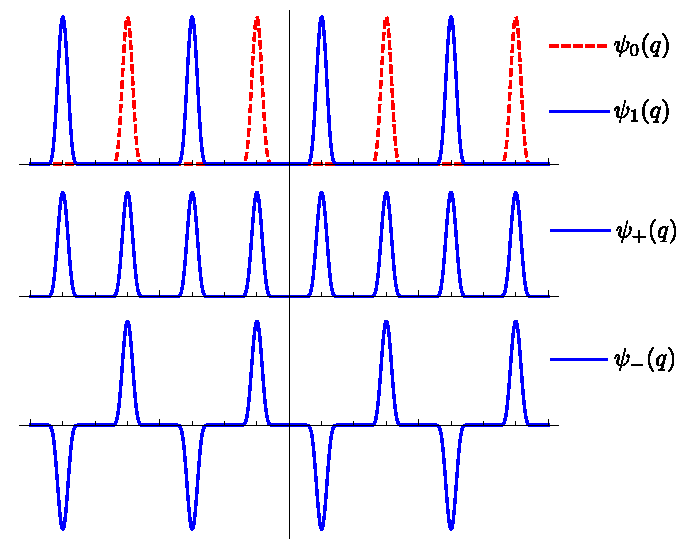
\includegraphics[width=10cm]{images/waveFunctions}
\end{frame}

\begin{frame}{Determinism in phase space (1/3)}




Was able to make good progress today. So here's what I did. First
of all, consider the same states $\left|\psi_{0}\right\rangle ,\left|\psi_{1}\right\rangle $
for $N=8$, as those considered in my first paper. Recall that for
$\hat{Z}$ as defined there, viz. $\hat{Z}=Z(\hat{q}_{\mod2L})$,
or more precisely as $\hat{Z}=Z(\hat{q})=\text{sgn}(\sin(\hat{q}\pi/L))$,
we had $\hat{Z}\left|\psi_{0}\right\rangle =\left|\psi_{0}\right\rangle $
and $\hat{Z}\left|\psi_{1}\right\rangle =-\left|\psi_{1}\right\rangle $.
In addition to this, I define $\hat{X}=e^{-i\hat{p}L/\hbar}$ (as
opposed to defining it to be hermitian). Now, we know that$\left|\psi_{\pm}\right\rangle \equiv\frac{\left|\psi_{0}\right\rangle +\left|\psi_{1}\right\rangle }{\sqrt{2}}$
is not an eigenstate of $\hat{X}$. So we optimize the observable
$\hat{X}$ to $\hat{X}'\equiv\hat{X}\hat{T}$, where $\hat{T}\equiv e^{i\hat{p}NLa(\hat{q})/2}$
where 
\[
a(q)=\begin{cases}
1 & 2L<q<4L\\
0 & \text{else}
\end{cases}.
\]
The idea is that you shift certain peaks to the right place, before
applying the displacement operator $\hat{X}$. 

\end{frame}

\begin{frame}{Determinism in phase space (2/3)}


To illustrate this, consider explicitly $\left|\psi_{0}\right\rangle =\left(\left|\varphi_{-4}\right\rangle +\left|\varphi_{-2}\right\rangle +\left|\varphi_{-1}\right\rangle +\left|\varphi_{-3}\right\rangle \right)/\sqrt{4}$.
The operation of $\hat{T}$ is $\hat{T}\left|\varphi_{4}\right\rangle =\left|\varphi_{-5}\right\rangle $,
$\hat{T}\left|\varphi_{3}\right\rangle =\left|\varphi_{-6}\right\rangle $
and $\hat{T}\left|\varphi_{n}\right\rangle =\left|\varphi_{n}\right\rangle $
for $n\in\{-4,-3,-2,-1,1,2\}$. It is now evident that $\hat{X}'=\hat{X}\hat{T}\left|\psi_{0}\right\rangle =\left|\psi_{1}\right\rangle $.
Note also that $\hat{X}'^{\dagger}\left|\psi_{0}\right\rangle =\left|\psi_{1}\right\rangle $.
Similarly $\hat{X}'\left|\psi_{1}\right\rangle =\left|\psi_{0}\right\rangle $
and $\hat{X}'^{\dagger}$ does the same. So finally, now consider
$\left|G\right\rangle \equiv\left(\left|\psi_{0}\psi_{0}\psi_{0}\right\rangle -\left|\psi_{1}\psi_{1}\psi_{1}\right\rangle \right)/\sqrt{2}$.
With $\hat{A}\equiv\hat{X}'\otimes\hat{Y}'\otimes\hat{Y}'^{\dagger}$,
where $\hat{Y}'\equiv i\hat{Z}\hat{X}'$, calculations yield $\hat{A}\left|G\right\rangle =\left|G\right\rangle $.
With $\hat{B}\equiv\hat{Y}'^{\dagger}\otimes\hat{X}'\otimes\hat{Y}'$
and $\hat{C}\equiv\hat{Y}'\otimes\hat{Y}'^{\dagger}\otimes\hat{X}'$
also, by symmetry we get $\hat{B}\left|G\right\rangle =\left|G\right\rangle $
and $\hat{C}\left|G\right\rangle =\left|G\right\rangle $. Now $\hat{D}\equiv\hat{A}\hat{B}\hat{C}=\hat{X}'\otimes\hat{Y}'\hat{X}\hat{Y}'^{\dagger}\otimes\hat{X}'$
and $\hat{E}\equiv\hat{X}'\otimes\hat{X}'\otimes\hat{X}'$ yield the
paradox. If values were predefined, the value of $\hat{D}$ and $\hat{E}$
would return the same answer. However, a simple calculation yields
$\hat{D}\left|G\right\rangle =\left|G\right\rangle $ (this can be
seen directly by applying $\hat{A},\,\hat{B}$ and $\hat{C}$ sequentially
on $\left|G\right\rangle $ {[}was figured the next day{]}), while
$\hat{E}\left|G\right\rangle =-\left|G\right\rangle $. 


\end{frame}

\begin{frame}{Determinism in phase space (3/3)}

\begin{itemize}
\item The GHZ argument entails then, that no theory can have $q,p$ NC deterministic.
\end{itemize}

\pause{}
\begin{itemize}
\item Counterexample: BM, a theory which is NC deterministic, in $q,p$.
\end{itemize}
\end{frame}

\begin{frame}{}



Bohmian Mechanics (BM) \\
Determinism: The GHZ test \& Contextuality \\
Analysis using BM  \\
(recent) Determinism in phase space $(q,p)$ \\
{\Huge {(in progress) Its analysis using BM}}

\end{frame}

\begin{frame}{BM analysis of GHZ 2.0}

\begin{itemize}
\item Measuring $\hat{X}'$ is not trivial.


\pause{}
\begin{itemize}
\item Wigner function
\end{itemize}

\pause{}
\begin{itemize}
\item Functions of $q,p$ directly from the particles $q,p$
\end{itemize}

\pause{}
\begin{itemize}
\item Formal measurement
\end{itemize}
\item Formally, any Hermitian operator can be measured using the interaction
Hamiltonian,$\hat{H}=-a\hat{Q}\hat{p}_{y}$, where $\hat{Q}$ is the
operator, and $y$ is the coordinate of the pointer.
\end{itemize}
\end{frame}

\begin{frame}{Conclusion}

\begin{itemize}
\item New insight into relation between contextuality and non locality
\item Fundamental difference between spins and $(q,p)$
\item Meaning of measurement
\item Pointed out and (almost) solved a paradox
\end{itemize}
\end{frame}

\begin{frame}{The End}


\Huge{Questions}

\end{frame}

\begin{frame}{References}


\nocite{*}
\bibliography{summary}

\end{frame}
\url{http://thisquantumworld.com/wp/wp-content/uploads/2015/01/surreal-1024x586-1024x586.png}
\end{document}
